% =====================================================================
%  Skripsi — Cipta Fikri Wiratama
%  Departemen Informatika, FSM, Universitas Diponegoro
%  Format: 02. Template dan Format Penulisan Skripsi V. 2024.10
%  Build : make   (xelatex + biber)
% =====================================================================
\documentclass[12pt,a4paper,oneside]{report}
\usepackage{undipskripsi}
\addbibresource{references.bib}

% ---------------- Data skripsi (ubah di sini) -------------------------
\judul{Pengembangan Chatbot Layanan Akademik dan Kemahasiswaan pada Sistem E-Office Menggunakan \textit{Process-Aware Workflow} GraphRAG (Studi Kasus: FSM UNDIP)}
\penulis{Cipta Fikri Wiratama}
\nim{24060122XXXXXX}% TODO: isi NIM
\tahun{2026}
\pembimbingsatu{Dr. Indra Waspada, S.T., M.T.I.}{NIP. ........................}% TODO: cek gelar dan NIP
\pembimbingdua{.....................................}{NIP. ........................}% TODO: pembimbing 2 (jika ada)
\tanggalpernyataan{.. ........ 2026}

% Nama-nama yang sering dipakai
\newcommand{\wgr}{\textit{Process-Aware Workflow} GraphRAG}
\newcommand{\eoffice}{E-Office}
\newcommand{\code}[1]{\texttt{#1}}

\begin{document}

% =================== BAGIAN AWAL (romawi kecil) =======================
\pagenumbering{roman}
% ---------------- SAMPUL (halaman i, nomor tidak ditampilkan) ----------
\begin{titlepage}
\centering\bfseries\setstretch{1.43}
ASISTEN VIRTUAL BERBASIS \textit{PROCESS-AWARE}\\
\textit{WORKFLOW} GRAPHRAG UNTUK LAYANAN PERSURATAN\\
AKADEMIK PADA SISTEM E-OFFICE\\
(Studi Kasus: Fakultas Sains dan Matematika\\
Universitas Diponegoro)

\vfill

\includegraphics[width=4.0cm,height=4.4cm]{img/logo-undip.png}
\vfill

SKRIPSI

\vfill
Disusun Sebagai Salah Satu Syarat\\
untuk Memperoleh Gelar Sarjana Komputer\\
pada Program Studi Informatika

\vfill
Disusun oleh:\\
\thepenulis\\
\thenim

\vfill
DEPARTEMEN INFORMATIKA\\
FAKULTAS SAINS DAN MATEMATIKA\\
UNIVERSITAS DIPONEGORO\\
2026
\end{titlepage}
\setcounter{page}{2}

% ---------------- HALAMAN PERNYATAAN KEASLIAN SKRIPSI ------------------
\frontchapter{HALAMAN PERNYATAAN KEASLIAN SKRIPSI}
\noindent Saya yang bertanda tangan di bawah ini :

\noindent\begin{tabularx}{\linewidth}{@{}l@{\ :\ }Y@{}}
Nama  & \thepenulis \\
NIM   & \thenim \\
Judul & \thejudul
\end{tabularx}

\vspace{6pt}
Dengan ini saya menyatakan bahwa dalam skripsi ini tidak terdapat karya yang pernah diajukan untuk memperoleh gelar kesarjanaan di suatu Perguruan Tinggi, dan sepanjang pengetahuan saya juga tidak terdapat karya atau pendapat yang pernah ditulis atau diterbitkan oleh orang lain, kecuali yang secara tertulis diacu dalam naskah ini dan disebutkan di dalam daftar pustaka.

\vspace{12pt}
\hfill\begin{tabular}{l}
Semarang, \thetanggal\\[4pt]
\fbox{\parbox[c][1.3cm][c]{2cm}{\centering\setstretch{1}\small Materai\\Rp 10.000,-}}\\[4pt]
\underline{\thepenulis}\\
\thenim
\end{tabular}
\clearpage

% ---------------- HALAMAN PENGESAHAN -----------------------------------
\frontchapter{HALAMAN PENGESAHAN}
\noindent\begin{tabularx}{\linewidth}{@{}l@{\ :\ }Y@{}}
Judul & \thejudul \\
Nama  & \thepenulis \\
NIM   & \thenim
\end{tabularx}

\vspace{6pt}
\noindent Telah diujikan pada sidang tugas akhir dan dinyatakan lulus pada tanggal \dotfill

\vspace{12pt}
\noindent\begin{tabular}{@{}p{0.5\linewidth}p{0.45\linewidth}@{}}
 & Semarang, ................ 2026\\
Pembimbing 1, & Pembimbing 2,\\[2.2cm]
\underline{\thepbsatu} & \underline{\thepbdua}\\
\thepbsatunip & \thepbduanip
\end{tabular}

\vspace{12pt}
\centerline{Mengetahui,}
\noindent\begin{tabular}{@{}p{0.5\linewidth}p{0.45\linewidth}@{}}
Ketua & Ketua\\
Departemen Informatika & Panitia Penguji Tugas Akhir\\[2.2cm]
\underline{Dr. Aris Sugiharto, S.Si., M.Kom.} & ...................................\\
NIP. 19710811 199702 1 004 & NIP.
\end{tabular}
\clearpage

% ---------------- KATA PENGANTAR ---------------------------------------
\frontchapter{KATA PENGANTAR}
Puji syukur penulis panjatkan ke hadirat Tuhan Yang Maha Esa atas rahmat dan karunia-Nya sehingga penulis dapat menyelesaikan skripsi yang berjudul ``\thejudul''. Skripsi ini disusun sebagai salah satu syarat untuk memperoleh gelar Sarjana Komputer pada Departemen Informatika, Fakultas Sains dan Matematika, Universitas Diponegoro.

Dalam penyusunan skripsi ini penulis mendapatkan bimbingan, bantuan, dan dukungan dari berbagai pihak. Oleh karena itu, penulis menyampaikan terima kasih kepada:
\begin{enumerate}
\item Dr. Aris Sugiharto, S.Si., M.Kom., selaku Ketua Departemen Informatika Fakultas Sains dan Matematika Universitas Diponegoro.
\item Dr. Indra Waspada, S.T., M.T.I., selaku dosen pembimbing yang telah meluangkan waktu untuk memberikan arahan dan masukan selama penelitian.
\item Seluruh dosen dan staf Departemen Informatika serta staf administrasi Fakultas Sains dan Matematika yang telah membantu penyediaan data dan informasi penelitian.
\item Keluarga dan rekan-rekan yang selalu memberikan dukungan.
\end{enumerate}

Penulis menyadari bahwa skripsi ini masih memiliki kekurangan. Oleh karena itu, kritik dan saran yang membangun sangat penulis harapkan. Semoga skripsi ini dapat bermanfaat bagi pembaca dan bagi pengembangan layanan administrasi akademik.

\vspace{12pt}
\hfill\begin{tabular}{c}
Semarang, .. ........ 2026\\[1.6cm]
Penulis
\end{tabular}
\clearpage

% ---------------- HALAMAN PERNYATAAN PERSETUJUAN PUBLIKASI -------------
\chapter*{HALAMAN PERNYATAAN PERSETUJUAN PUBLIKASI SKRIPSI\protect\\ UNTUK KEPENTINGAN AKADEMIS}
\addcontentsline{toc}{chapter}{HALAMAN PERNYATAAN PERSETUJUAN PUBLIKASI SKRIPSI}
\noindent Sebagai civitas akademik Universitas Diponegoro, saya yang bertanda tangan di bawah ini:

\noindent\begin{tabularx}{\linewidth}{@{}l@{\ :\ }Y@{}}
Nama          & \thepenulis \\
NIM           & \thenim \\
Program Studi & Informatika \\
Departemen    & Informatika \\
Fakultas      & Sains dan Matematika \\
Jenis Karya   & Skripsi
\end{tabularx}

\noindent demi pengembangan ilmu pengetahuan, menyetujui untuk memberikan Hak Bebas Royalti Noneksklusif (\textit{Non-exclusive Royalty Free Right}) kepada Universitas Diponegoro atas karya ilmiah saya yang berjudul:

\begin{center}\thejudul\end{center}

\noindent beserta perangkat yang ada (jika diperlukan). Dengan Hak Bebas Royalti Noneksklusif ini Universitas Diponegoro berhak menyimpan, mengalihmedia/formatkan, mengelola dalam bentuk pangkalan data (\textit{database}), merawat, dan mempublikasikan skripsi saya tanpa meminta izin dari saya selama tetap mencantumkan nama saya sebagai penulis/pencipta dan sebagai pemilik Hak Cipta.

Demikian pernyataan ini saya buat dengan sebenarnya.

\vspace{12pt}
\hfill\begin{tabular}{l}
Semarang, .. ........ 2026\\[1.8cm]
\underline{\thepenulis}\\
\thenim
\end{tabular}
\clearpage

% ---------------- ABSTRAK (maks. 300 kata, satu spasi, tanpa indentasi) --
% TODO: perbarui hasil setelah Bab IV selesai.
\frontchapter{ABSTRAK}
\begingroup\setstretch{1}\setlength{\parindent}{0pt}
Layanan administrasi akademik di Fakultas Sains dan Matematika (FSM) Universitas Diponegoro dijalankan berdasarkan Standar Operasional Prosedur (SOP), sehingga staf tata usaha menerima banyak pertanyaan berulang mengenai urutan langkah, pejabat yang bertanggung jawab, dan dokumen persyaratan. Asisten virtual berbasis \textit{Large Language Model} (LLM) dapat menjawab pertanyaan tersebut, tetapi LLM berbasis \textit{cloud} menimbulkan biaya per kueri dan risiko kebocoran data mahasiswa, sedangkan \textit{Retrieval-Augmented Generation} (RAG) konvensional cenderung mencampurkan langkah dari SOP yang berbeda dan membalik urutan langkah. Penelitian ini mengembangkan asisten virtual yang terintegrasi dengan sistem persuratan digital E-Office dan menggunakan mesin \textit{Process-Aware Workflow} GraphRAG. Setiap SOP dimodelkan sebagai graf alur kerja berarah yang menyimpan aktor, aksi, dokumen masukan, keluaran, dan durasi setiap langkah. Pemilih SOP berbasis aturan menentukan prosedur yang relevan, langkah-langkahnya diserialisasi secara berurutan, lalu dilengkapi potongan dokumen pendukung sebelum dijawab oleh LLM lokal \texttt{gemma4:e2b} melalui Ollama. Alur percakapan diorkestrasi menggunakan LangGraph dan disajikan melalui antarmuka E-Office berbasis Next.js dengan layanan \textit{backend} Bun dan Elysia. Evaluasi menggunakan 40 pertanyaan terverifikasi dengan metrik \textit{key-fact recall} (KFR), cakupan langkah, \textit{Topological Inversion Rate} (TIR), \textit{Actor Mismatch Rate} (AMR), akurasi penolakan, dan efisiensi token, dilengkapi pengujian \textit{black-box} terhadap fitur sistem. Pengujian pendahuluan menunjukkan bahwa mesin tersebut mencapai KFR 0,955 dibandingkan 0,712 pada Naive RAG, cakupan langkah 1,000, TIR 0,000, dan menggunakan 44\% lebih sedikit token prompt dibandingkan pemberian seluruh dokumen. Hasil ini menunjukkan bahwa pemilihan prosedur dan representasi alur kerja yang eksplisit memungkinkan LLM berukuran kecil yang berjalan secara lokal memberikan jawaban prosedural yang lengkap dan berurutan.

\vspace{12pt}
\noindent Kata kunci : \textit{Retrieval-Augmented Generation}, GraphRAG, graf alur kerja, SOP, E-Office, asisten virtual, LLM lokal
\par\endgroup
\clearpage

% ---------------- ABSTRACT (tidak ditulis miring) -----------------------
\begin{otherlanguage}{american}
\chapter*{ABSTRACT}\addcontentsline{toc}{chapter}{ABSTRACT}
\begingroup\setstretch{1}\setlength{\parindent}{0pt}
Academic administration at the Faculty of Science and Mathematics (FSM), Universitas Diponegoro, follows Standard Operating Procedures (SOPs), so administrative staff receive many repeated questions about step order, responsible officials, and required documents. A virtual assistant based on a Large Language Model (LLM) can answer such questions, but cloud-hosted LLMs add per-query costs and risk exposing student data, while conventional Retrieval-Augmented Generation (RAG) tends to mix steps from different SOPs and reverse their order. This research develops a virtual assistant integrated into the E-Office digital correspondence system and powered by a Process-Aware Workflow GraphRAG engine. Each SOP is modelled as a directed workflow graph that stores the actor, action, input documents, outputs, and duration of every step. A rule-based selector identifies the relevant procedure, its steps are serialized in order and complemented with supporting document chunks, and a local LLM, gemma4:e2b served through Ollama, generates the answer. The conversation flow is orchestrated with LangGraph and delivered through the Next.js E-Office interface with a Bun and Elysia backend. Evaluation uses 40 verified questions with key-fact recall (KFR), step coverage, Topological Inversion Rate (TIR), Actor Mismatch Rate (AMR), refusal accuracy, and token efficiency, complemented by black-box testing of system features. Preliminary tests show that the engine reaches a KFR of 0.955 compared with 0.712 for Naive RAG, a step coverage of 1.000 and a TIR of 0.000, while using 44\% fewer prompt tokens than supplying every document. These results indicate that procedure selection and an explicit workflow representation allow a small, locally hosted LLM to give complete and correctly ordered procedural answers.

\vspace{12pt}
\noindent Keywords : Retrieval-Augmented Generation, GraphRAG, workflow graph, SOP, E-Office, virtual assistant, local LLM
\par\endgroup
\end{otherlanguage}
\clearpage


\begingroup
\setstretch{1.43}
\clearpage
\phantomsection\addcontentsline{toc}{chapter}{DAFTAR ISI}
\tableofcontents
\clearpage
\phantomsection\addcontentsline{toc}{chapter}{DAFTAR TABEL}
\listoftables
\clearpage
\phantomsection\addcontentsline{toc}{chapter}{DAFTAR GAMBAR}
\listoffigures
\endgroup

% =================== BAGIAN INTI (arab, mulai 1) =======================
\cleardoublepage
\pagenumbering{arabic}
% =====================================================================
\chapter{Pendahuluan}
\label{bab:1}
% =====================================================================
Bab pendahuluan ini membahas mengenai latar belakang masalah, rumusan masalah, tujuan dan manfaat, ruang lingkup, serta sistematika penulisan yang digunakan dalam dokumen skripsi ini.

\section{Latar Belakang}
\label{sec:latar}
Layanan administrasi akademik di Fakultas Sains dan Matematika (FSM) Universitas Diponegoro, seperti izin cuti akademik, permohonan aktif kembali setelah cuti, legalisir ijazah dan transkrip, pengisian Isian Rencana Studi (IRS), izin keterlambatan pembayaran Uang Kuliah Tunggal (UKT), rekomendasi beasiswa, dan pengajuan proposal kegiatan organisasi mahasiswa, dijalankan berdasarkan Standar Operasional Prosedur (SOP). Setiap SOP menetapkan urutan langkah, pejabat atau unit yang melaksanakan setiap langkah, dokumen yang dibutuhkan, dan keluaran yang dihasilkan. Mahasiswa yang tidak memahami SOP cenderung bertanya berulang kali kepada staf tata usaha tentang hal yang sama, sehingga waktu staf tersita untuk menjawab pertanyaan rutin dan mahasiswa harus menunggu jam layanan untuk memperoleh jawaban.

Sebagian layanan tersebut berujung pada pengajuan surat, misalnya surat permohonan cuti atau surat rekomendasi beasiswa. Untuk itu, penulis mengembangkan sistem persuratan digital E-Office yang memindahkan pengajuan surat dari kertas ke alur elektronik, sejalan dengan arah Sistem Pemerintahan Berbasis Elektronik \parencite{perpres95_2018}. Setiap surat di E-Office bergerak melalui status yang berurutan, yaitu \code{SUBMITTED}, \code{VERIFIED}, \code{SIGNED}, dan \code{REGISTERED}, dan diproses oleh aktor yang berbeda pada setiap tahap. Sistem ini mempercepat pemrosesan surat, tetapi belum menjawab pertanyaan mahasiswa tentang prosedur yang harus ditempuh sebelum dan selama surat diproses. Kebutuhan akan kanal tanya jawab yang tersedia setiap saat dan terhubung langsung dengan E-Office menjadi dasar pengembangan asisten virtual dalam penelitian ini.

Asisten virtual berbasis \textit{Large Language Model} (LLM) mampu memahami pertanyaan dalam bahasa alami dan menyusun jawaban yang luwes \parencite{brown2020gpt3}. Namun, LLM dapat menghasilkan informasi yang tampak meyakinkan tetapi tidak sesuai fakta \parencite{ji2023hallucination}, dan LLM berbasis \textit{cloud} menimbulkan biaya per kueri serta mengirim data mahasiswa ke pihak ketiga. LLM berukuran kecil (2 hingga 5 miliar parameter) yang dijalankan secara lokal menghindari kedua masalah tersebut, tetapi lebih mudah terganggu oleh konteks yang tidak relevan \parencite{liu2024lost}. Dalam jawaban administratif, kesalahan kecil berdampak nyata: langkah yang tertukar, pejabat yang salah, atau dokumen yang terlewat membuat mahasiswa datang ke loket yang salah.

\textit{Retrieval-Augmented Generation} (RAG) mengurangi masalah tersebut dengan menyertakan potongan dokumen yang relevan ke dalam \textit{prompt} sebelum LLM menjawab \parencite{lewis2020rag,gao2023ragsurvey}. Penelitian sebelumnya di FSM telah menerapkan RAG pada chatbot layanan kemahasiswaan dan membandingkannya dengan RASA \parencite{sutantio2026perbandingan}, serta menggabungkan keduanya dalam chatbot hibrida berbasis web \parencite{sahnah2026pengembangan}. Kedua penelitian tersebut memperlakukan SOP sebagai teks biasa. Karena SOP FSM pendek, setiap SOP menjadi satu potongan dokumen, sehingga pencarian tiga potongan teratas selalu memasukkan tiga SOP utuh yang memakai kosakata serupa (misalnya dekan, subbagian akademik, verifikasi, dan tanda tangan). Akibatnya, LLM harus memisahkan prosedur yang saling bersaing dan berisiko mencampurkan langkah dari SOP lain atau membalik urutan langkah. GraphRAG menambahkan struktur graf pada proses temu kembali \parencite{peng2024graphragsurvey,edge2024graphrag}, tetapi graf yang umum digunakan adalah graf entitas-relasi \parencite{guo2024lightrag,gutierrez2024hipporag} yang tidak menyimpan urutan eksekusi maupun aktor pada setiap langkah.

Penelitian pendahuluan penulis bersama pembimbing mengusulkan \wgr{}, yaitu pendekatan yang memodelkan setiap SOP sebagai graf alur kerja berarah \parencite{dumas2018fundamentals}, memilih SOP target dengan pemilih berbasis aturan, lalu menyerahkan langkah-langkah yang berurutan kepada LLM lokal \parencite{wiratama2026procedure}. Pada 40 pertanyaan terverifikasi, pendekatan ini mencapai \textit{key-fact recall} 0,955 dibandingkan 0,712 pada Naive RAG, cakupan langkah 1,000 tanpa pembalikan urutan, dan menggunakan 44\% lebih sedikit token \textit{prompt} dibandingkan pemberian seluruh SOP. Studi ablasi pada penelitian tersebut juga menunjukkan bahwa peningkatan kelengkapan jawaban terutama berasal dari pemilihan SOP yang tepat, sedangkan graf alur kerja memberikan urutan yang konsisten, atribusi aktor yang eksplisit, dan \textit{prompt} yang lebih ringkas. Penelitian tersebut masih berupa eksperimen terhadap mesin RAG dan belum diterapkan sebagai layanan yang dapat digunakan mahasiswa.

Berdasarkan uraian tersebut, penelitian ini mengembangkan asisten virtual untuk layanan persuratan akademik yang terintegrasi dengan sistem E-Office dan menggunakan \wgr{} sebagai mesin tanya jawabnya. Asisten virtual dijalankan dengan LLM lokal agar data mahasiswa tetap berada di lingkungan kampus, diorkestrasi menggunakan LangGraph \parencite{langgraph2024}, dan dievaluasi dengan metrik prosedural yang mengukur kelengkapan, urutan, dan ketepatan aktor pada jawaban, serta pengujian fungsional terhadap sistem.

\section{Rumusan Masalah}
\label{sec:rumusan}
Berdasarkan latar belakang yang telah diuraikan, rumusan masalah dalam penelitian ini sebagai berikut:
\begin{enumerate}
\item Bagaimana membangun asisten virtual yang terintegrasi dengan sistem E-Office dan menggunakan \wgr{} untuk menjawab pertanyaan mahasiswa tentang SOP layanan akademik FSM?
\item Bagaimana kualitas jawaban asisten virtual, yang diukur dengan \textit{key-fact recall}, cakupan langkah, \textit{Topological Inversion Rate}, \textit{Actor Mismatch Rate}, dan akurasi penolakan, dibandingkan dengan RAG berbasis potongan teks dan GraphRAG berbasis entitas?
\item Bagaimana efisiensi asisten virtual dalam hal jumlah token \textit{prompt} dan waktu respons ketika dijalankan dengan LLM lokal?
\end{enumerate}

\section{Tujuan dan Manfaat}
\label{sec:tujuan-manfaat}
Subbab ini menguraikan tujuan yang ingin dicapai melalui penelitian serta manfaat yang diharapkan bagi pihak-pihak terkait.

\subsection{Tujuan Penelitian}
Tujuan penelitian ini sebagai berikut:
\begin{enumerate}
\item Menghasilkan asisten virtual layanan persuratan akademik yang terintegrasi dengan sistem E-Office dan menggunakan \wgr{} dengan LLM lokal.
\item Mengukur kualitas jawaban prosedural asisten virtual dan membandingkannya dengan Naive RAG serta GraphRAG berbasis entitas menggunakan benchmark pertanyaan yang terverifikasi.
\item Mengukur efisiensi token \textit{prompt} dan waktu respons asisten virtual sebagai dasar kelayakan penerapan di lingkungan fakultas.
\end{enumerate}

\subsection{Manfaat Penelitian}
Manfaat yang diharapkan dari penelitian ini sebagai berikut:
\begin{enumerate}
\item Bagi mahasiswa, asisten virtual menyediakan informasi prosedur layanan akademik yang lengkap, berurutan, dan dapat diakses setiap saat langsung dari E-Office.
\item Bagi staf administrasi FSM, asisten virtual mengurangi beban menjawab pertanyaan berulang sehingga staf dapat berfokus pada pemrosesan surat.
\item Bagi fakultas, penggunaan LLM lokal menjaga data mahasiswa tetap berada di lingkungan kampus dan menghindari biaya layanan LLM berbasis \textit{cloud}.
\item Bagi bidang keilmuan, penelitian ini memberikan contoh penerapan GraphRAG berbasis alur kerja pada sistem nyata beserta evaluasi prosedural yang dapat direplikasi.
\end{enumerate}

\section{Ruang Lingkup}
\label{sec:ruang-lingkup}
Ruang lingkup penelitian ini sebagai berikut:
\begin{enumerate}
\item Basis pengetahuan terdiri atas 7 SOP layanan mahasiswa yang diterbitkan FSM Universitas Diponegoro, yaitu izin cuti akademik, permohonan aktif kembali setelah cuti, legalisir ijazah dan transkrip, pengisian IRS, izin keterlambatan pembayaran UKT, rekomendasi beasiswa, dan pengajuan proposal kegiatan organisasi mahasiswa. % TODO: konfirmasi bahwa SOP persuratan E-Office sama dengan korpus paper
\item Graf alur kerja disusun secara manual dari dokumen SOP dan diimplementasikan menggunakan NetworkX \parencite{hagberg2008networkx}.
\item LLM utama yang digunakan adalah \texttt{gemma4:e2b} yang dijalankan secara lokal melalui Ollama \parencite{ollama2023}; satu LLM lokal lain digunakan sebagai pembanding.
\item Asisten virtual hanya menjawab pertanyaan berbahasa Indonesia yang berkaitan dengan ketujuh SOP serta status surat milik pengguna di E-Office, dan menolak pertanyaan di luar cakupan tersebut.
\item Asisten virtual diintegrasikan ke sistem E-Office yang dibangun dengan Next.js pada sisi antarmuka serta Bun dan Elysia pada sisi \textit{backend}, dengan basis data PostgreSQL.
\item Evaluasi kualitas jawaban menggunakan benchmark 40 pertanyaan terverifikasi yang terdiri atas 35 pertanyaan yang dapat dijawab dan 5 pertanyaan di luar cakupan, sedangkan evaluasi fungsional menggunakan pengujian \textit{black-box}.
\end{enumerate}

\section{Sistematika Penulisan}
\label{sec:sistematika}
Sistematika penulisan skripsi ini sebagai berikut:
\begin{enumerate}
\item BAB I PENDAHULUAN\\
Bab ini membahas latar belakang, rumusan masalah, tujuan dan manfaat, ruang lingkup, serta sistematika penulisan skripsi.
\item BAB II TINJAUAN PUSTAKA\\
Bab ini membahas penelitian terkait serta dasar teori yang digunakan, meliputi sistem E-Office dan SOP, chatbot, LLM, RAG, GraphRAG, pemodelan proses bisnis, \wgr{}, teknologi yang digunakan, dan metode evaluasi.
\item BAB III METODOLOGI PENELITIAN\\
Bab ini membahas tahapan penelitian, mulai dari pengumpulan data, analisis kebutuhan, perancangan, implementasi, hingga pengujian dan evaluasi, serta jadwal penelitian.
\item BAB IV HASIL DAN PEMBAHASAN\\
Bab ini membahas hasil implementasi asisten virtual, hasil evaluasi kualitas jawaban dan efisiensi, hasil pengujian fungsional, serta pembahasannya.
\item BAB V PENUTUP\\
Bab ini berisi kesimpulan dari hasil penelitian dan saran untuk penelitian selanjutnya.
\end{enumerate}

% =====================================================================
\chapter{Tinjauan Pustaka}
\label{bab:2}
% =====================================================================
Bab ini membahas penelitian terkait dan dasar teori yang digunakan dalam penelitian, meliputi sistem E-Office dan SOP layanan akademik, chatbot dan asisten virtual, \textit{Large Language Model}, \textit{Retrieval-Augmented Generation}, GraphRAG, pemodelan proses bisnis, \wgr{}, teknologi yang digunakan, serta metode evaluasi.

% ---------------------------------------------------------------------
\section{Penelitian Terkait}
\label{sec:terkait}
Penelitian terkait yang menjadi acuan dalam skripsi ini ditunjukkan pada Tabel~\ref{tab:terkait}. Penelitian-penelitian tersebut dikelompokkan berdasarkan objek studi dan pendekatan yang digunakan.

\begin{table}[htbp]
\caption{Penelitian Terkait}
\label{tab:terkait}
\centering\tabsetup
\begin{tabularx}{\linewidth}{|C{0.6cm}|L{3.0cm}|Y|L{3.6cm}|}
\hline\hdr
\hrow\textbf{No} & \textbf{Peneliti} & \textbf{Pendekatan dan Hasil} & \textbf{Keterbatasan} \\\hline
1 & \textcite{sutantio2026perbandingan} & Membandingkan RASA dan RAG pada chatbot layanan kemahasiswaan FSM dengan 7 SOP yang sama. Akurasi keduanya tidak berbeda signifikan, RASA jauh lebih cepat, sedangkan RAG lebih mudah disiapkan. & SOP diperlakukan sebagai teks; urutan langkah dan aktor tidak diukur. \\\hline
2 & \textcite{sahnah2026pengembangan} & Chatbot hibrida NLU-RASA dan LLM-RAG berbasis web (Next.js dan FastAPI) dengan metodologi ICONIX, diuji oleh responden mahasiswa. & Fokus pada rekayasa perangkat lunak; tidak ada evaluasi prosedural. \\\hline
3 & \textcite{lewis2020rag} & Memperkenalkan RAG yang menggabungkan \textit{retriever} padat dengan generator sekuens. & Konteks berupa teks tidak terstruktur. \\\hline
4 & \textcite{edge2024graphrag}; \textcite{guo2024lightrag} & GraphRAG dan LightRAG membangun graf entitas-relasi dengan LLM untuk pertanyaan global dan lokal. & Tidak menyimpan urutan eksekusi langkah. \\\hline
5 & \textcite{lin2026soprag} & SOPRAG menggunakan pakar graf alur dan graf entitas untuk menemukan SOP industri. & Indeks dipelajari pada skala besar; efek pemilihan dan penstrukturan tidak dipisahkan. \\\hline
6 & \textcite{wiratama2026procedure} & \wgr{} pada 7 SOP FSM dengan LLM lokal; KFR 0,955 dan cakupan langkah 1,000; pemilihan SOP menjadi faktor utama. & Masih berupa eksperimen; belum diterapkan pada sistem layanan. \\\hline
\end{tabularx}
\end{table}

Berdasarkan Tabel~\ref{tab:terkait}, penelitian di FSM telah menerapkan chatbot untuk SOP layanan kemahasiswaan, tetapi belum memodelkan urutan langkah dan aktor secara eksplisit. Sebaliknya, penelitian pendahuluan penulis telah menguji representasi alur kerja tersebut, tetapi belum menerapkannya sebagai layanan. Skripsi ini mengisi celah tersebut dengan menerapkan \wgr{} sebagai mesin asisten virtual pada sistem E-Office.

% ---------------------------------------------------------------------
\section{Sistem E-Office dan SOP Layanan Akademik}
\label{sec:eoffice}
Subbab ini membahas sistem persuratan digital E-Office yang menjadi tempat penerapan asisten virtual, serta struktur dokumen SOP yang menjadi basis pengetahuannya.

\subsection{Sistem Persuratan Digital E-Office}
E-Office adalah sistem informasi yang mendigitalkan proses perkantoran, terutama pembuatan, verifikasi, penandatanganan, dan pengarsipan surat. Di Indonesia, penerapan sistem semacam ini merupakan bagian dari Sistem Pemerintahan Berbasis Elektronik (SPBE) yang mendorong layanan administrasi terpadu berbasis elektronik \parencite{perpres95_2018}. Pada lingkungan akademik, E-Office memungkinkan mahasiswa mengajukan surat secara daring dan memantau prosesnya tanpa harus datang ke loket.

Sistem E-Office yang dikembangkan penulis memodelkan setiap surat sebagai entitas yang berpindah status secara berurutan. Alur status surat dan aktor yang memprosesnya ditunjukkan pada Gambar~\ref{fig:eoffice-status}. Mahasiswa mengajukan surat (\code{SUBMITTED}), surat diverifikasi oleh SA (\code{VERIFIED}), ditandatangani oleh MTU (\code{SIGNED}), lalu dicatat dan diberi nomor oleh UPA (\code{REGISTERED}). % TODO: tulis kepanjangan SA, MTU, dan UPA
Alur ini juga merupakan alur kerja berarah, sehingga cocok dengan pendekatan graf alur kerja yang digunakan untuk SOP.

\begin{figure}[htbp]
\centering
\begin{tikzpicture}[font=\normalsize,
  st/.style={draw, rounded corners=3pt, minimum width=2.6cm, minimum height=1cm, align=center, fill=g8},
  ac/.style={font=\normalsize\itshape, align=center},
  arr/.style={-{Stealth[length=2.2mm]}, thick}]
\node[st] (s1) at (0,0)    {\code{SUBMITTED}};
\node[st] (s2) at (3.6,0)  {\code{VERIFIED}};
\node[st] (s3) at (7.2,0)  {\code{SIGNED}};
\node[st] (s4) at (10.8,0) {\code{REGISTERED}};
\draw[arr] (s1) -- (s2); \draw[arr] (s2) -- (s3); \draw[arr] (s3) -- (s4);
\node[ac, below=0.35cm of s1] {Mahasiswa\\mengajukan};
\node[ac, below=0.35cm of s2] {SA\\memverifikasi};
\node[ac, below=0.35cm of s3] {MTU\\menandatangani};
\node[ac, below=0.35cm of s4] {UPA\\mencatat};
\end{tikzpicture}
\caption{Alur Status Surat pada Sistem E-Office}
\label{fig:eoffice-status}
\end{figure}

\subsection{Standar Operasional Prosedur Layanan Akademik}
\label{sec:sop}
Standar Operasional Prosedur (SOP) adalah dokumen yang menetapkan langkah-langkah baku untuk menyelesaikan suatu layanan. FSM Universitas Diponegoro menerbitkan 7 SOP layanan mahasiswa yang masing-masing terdiri atas satu halaman berbahasa Indonesia dengan total 44 langkah bernomor \parencite{wiratama2026procedure}. Seluruh SOP berbentuk urutan linier tanpa percabangan. Struktur dokumen SOP ditunjukkan pada Gambar~\ref{fig:anatomi-sop}: judul, kalimat tujuan yang dapat memuat batas waktu pemrosesan, serta langkah bernomor yang subjek kalimatnya adalah pelaksana langkah, dan dapat diikuti baris \textit{Waktu}, \textit{Dokumen yang dibutuhkan}, dan \textit{Output}.

\begin{figure}[htbp]
\centering
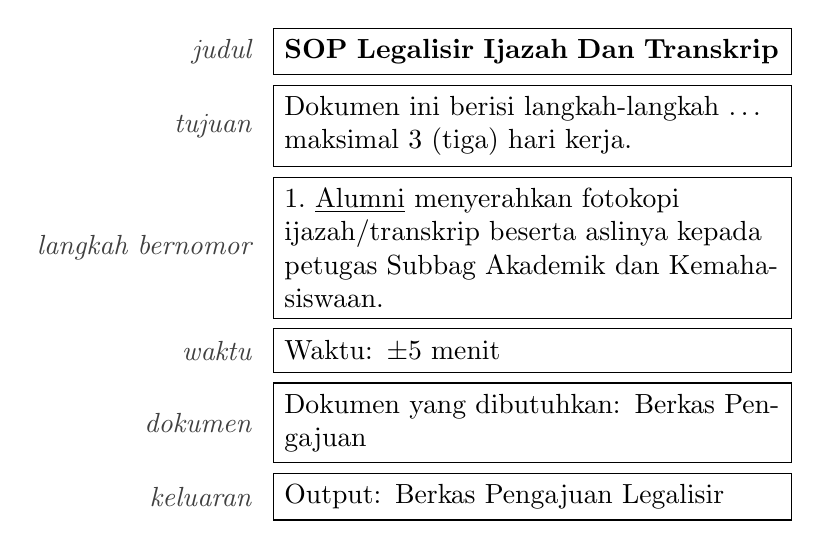
\begin{tikzpicture}[font=\normalsize,
  doc/.style={draw, fill=white, align=left, inner sep=1.4mm, text width=6.3cm},
  tag/.style={font=\normalsize\itshape, anchor=east, text=black!75}]
\node[doc] (title) at (0,0) {\textbf{SOP Legalisir Ijazah Dan Transkrip}};
\node[doc, anchor=north] (purp) at ([yshift=-1.2mm]title.south) {Dokumen ini berisi langkah-langkah \dots\ maksimal 3 (tiga) hari kerja.};
\node[doc, anchor=north] (step) at ([yshift=-1.2mm]purp.south) {1.\ \underline{Alumni} menyerahkan fotokopi ijazah/transkrip beserta aslinya kepada petugas Subbag Akademik dan Kemahasiswaan.};
\node[doc, anchor=north] (wkt) at ([yshift=-1.2mm]step.south) {Waktu: $\pm$5 menit};
\node[doc, anchor=north] (dok) at ([yshift=-1.2mm]wkt.south) {Dokumen yang dibutuhkan: Berkas Pengajuan};
\node[doc, anchor=north] (out) at ([yshift=-1.2mm]dok.south) {Output: Berkas Pengajuan Legalisir};
\node[tag] at ([xshift=-1.5mm]title.west) {judul};
\node[tag] at ([xshift=-1.5mm]purp.west) {tujuan};
\node[tag] at ([xshift=-1.5mm]step.west) {langkah bernomor};
\node[tag] at ([xshift=-1.5mm]wkt.west) {waktu};
\node[tag] at ([xshift=-1.5mm]dok.west) {dokumen};
\node[tag] at ([xshift=-1.5mm]out.west) {keluaran};
\end{tikzpicture}
\caption{Struktur Dokumen SOP FSM (Contoh Langkah 1 SOP Legalisir)}
\label{fig:anatomi-sop}
\end{figure}

Langkah-langkah SOP dilaksanakan oleh 15 peran organisasi, mulai dari mahasiswa, program studi, pimpinan fakultas, unit administrasi fakultas, hingga tingkat universitas. Mahasiswa melaksanakan 21 dari 44 langkah, dan beberapa peran fakultas terlibat di lebih dari satu SOP \parencite{wiratama2026procedure}. Akibatnya, SOP yang berbeda berbagi aktor dan kosakata yang sama, yang menyulitkan temu kembali berbasis kemiripan teks.

% ---------------------------------------------------------------------
\section{Chatbot dan Asisten Virtual}
\label{sec:chatbot}
Chatbot adalah program yang berinteraksi dengan pengguna melalui bahasa alami \parencite{adamopoulou2020overview}. Chatbot awal seperti ELIZA bekerja dengan pencocokan pola \parencite{weizenbaum1966eliza}, kemudian berkembang menjadi chatbot berbasis \textit{Natural Language Understanding} (NLU) yang mengklasifikasikan maksud (\textit{intent}) dan mengekstraksi entitas, seperti RASA. Asisten virtual generasi terbaru menggunakan LLM sehingga dapat menyusun jawaban baru tanpa harus menyiapkan seluruh pola percakapan terlebih dahulu \parencite{jurafsky2026slp}. Kelemahannya, jawaban LLM perlu dikendalikan agar tetap sesuai dengan sumber resmi, yang menjadi alasan penggunaan RAG pada penelitian ini.

% ---------------------------------------------------------------------
\section{Large Language Model}
\label{sec:llm}
Subbab ini membahas arsitektur dasar LLM serta penggunaan LLM berukuran kecil yang dijalankan secara lokal.

\subsection{Arsitektur Transformer}
LLM modern dibangun di atas arsitektur Transformer yang menggunakan mekanisme \textit{self-attention} untuk menghitung hubungan antartoken dalam satu urutan \parencite{vaswani2017attention}. Perhitungan \textit{attention} ditunjukkan pada Persamaan~\ref{eq:attention}:
\begin{equation}
\mathrm{Attention}(Q,K,V)=\mathrm{softmax}\!\left(\frac{QK^{\top}}{\sqrt{d_k}}\right)V
\label{eq:attention}
\end{equation}
\begin{keterangan}
$Q$ & Matriks \textit{query} hasil proyeksi representasi token \\
$K$ & Matriks \textit{key} hasil proyeksi representasi token \\
$V$ & Matriks \textit{value} hasil proyeksi representasi token \\
$d_k$ & Dimensi vektor \textit{key} \\
\end{keterangan}

Model yang dilatih pada korpus teks berskala besar dengan tujuan memprediksi token berikutnya mampu mengerjakan berbagai tugas hanya dengan instruksi dan sedikit contoh di dalam \textit{prompt} \parencite{brown2020gpt3}. Kemampuan inilah yang memungkinkan LLM digunakan sebagai generator jawaban pada asisten virtual.

\subsection{LLM Lokal}
LLM berbobot terbuka seperti LLaMA \parencite{touvron2023llama} dan Gemma \parencite{gemmateam2024gemma} dapat dijalankan pada perangkat milik institusi. Ollama menyediakan layanan untuk mengunduh, menjalankan, dan memanggil model tersebut melalui antarmuka HTTP lokal \parencite{ollama2023}. Penggunaan LLM lokal menghindari biaya per kueri dan menjaga data tetap di dalam jaringan kampus. Akan tetapi, model berukuran kecil memiliki kapasitas penalaran terbatas dan lebih mudah terganggu ketika konteks memuat banyak informasi yang tidak relevan \parencite{liu2024lost}. LLM juga dapat berhalusinasi, yaitu menghasilkan informasi yang tidak didukung sumber \parencite{ji2023hallucination}. Oleh karena itu, konteks yang diberikan kepada model kecil perlu ringkas dan tepat sasaran.

% ---------------------------------------------------------------------
\section{Retrieval-Augmented Generation}
\label{sec:rag}
\textit{Retrieval-Augmented Generation} (RAG) adalah pendekatan yang mengondisikan generator pada dokumen hasil temu kembali \parencite{lewis2020rag,church2024emerging}. Alur umum RAG ditunjukkan pada Gambar~\ref{fig:rag}. Pada tahap luring, dokumen dipotong, diubah menjadi vektor, dan disimpan dalam basis data vektor. Pada tahap daring, pertanyaan diubah menjadi vektor, potongan yang paling mirip diambil, lalu disusun bersama pertanyaan menjadi \textit{prompt} untuk LLM \parencite{gao2023ragsurvey}.

\begin{figure}[htbp]
\centering
\begin{tikzpicture}[font=\normalsize,
  box/.style={draw, rounded corners=2pt, align=center, minimum height=1.1cm, text width=2.2cm, fill=white},
  arr/.style={-{Stealth[length=2mm]}, thick},
  lane/.style={draw=g60, rounded corners=4pt, fill=g6, inner sep=2.5mm}]
\node[box] (d) at (0,0) {Dokumen\\SOP};
\node[box] (c) at (3.2,0) {\textit{Chunking}};
\node[box] (e) at (6.4,0) {Embedding};
\node[box] (v) at (9.6,0) {Basis data\\vektor};
\draw[arr] (d)--(c); \draw[arr] (c)--(e); \draw[arr] (e)--(v);
\node[box] (q) at (0,-2.6) {Pertanyaan};
\node[box] (r) at (3.2,-2.6) {Temu kembali\\top-$k$};
\node[box] (p) at (6.4,-2.6) {\textit{Prompt}:\\konteks + tanya};
\node[box] (g) at (9.6,-2.6) {LLM\\(generator)};
\draw[arr] (q)--(r); \draw[arr] (r)--(p); \draw[arr] (p)--(g);
\draw[arr] (v.south) -- ++(0,-0.55) -| (r.north);
\begin{scope}[on background layer]
\node[lane, fit=(d)(v)] (off) {};
\node[lane, fit=(q)(g)] (on) {};
\end{scope}
\node[anchor=south west, font=\normalsize\bfseries] at (off.north west) {Tahap luring (sekali)};
\node[anchor=north west, font=\normalsize\bfseries] at (on.south west) {Tahap daring (setiap pertanyaan)};
\end{tikzpicture}
\caption{Alur Umum \textit{Retrieval-Augmented Generation}}
\label{fig:rag}
\end{figure}

\subsection{Chunking}
\textit{Chunking} adalah proses memecah dokumen menjadi potongan yang dapat dicari. Ukuran potongan menentukan keseimbangan antara kelengkapan konteks dan ketepatan temu kembali. Pada penelitian pendahuluan, dokumen dipotong dengan jendela 1.700 karakter dan tumpang tindih 100 karakter. Karena setiap SOP FSM lebih pendek dari 1.650 karakter, setiap SOP menjadi tepat satu potongan, sehingga pencarian tiga potongan teratas selalu memasukkan tiga SOP utuh ke dalam \textit{prompt} \parencite{wiratama2026procedure}.

\subsection{Embedding Teks}
\textit{Embedding} adalah representasi teks dalam bentuk vektor berdimensi tetap yang menempatkan teks bermakna serupa pada posisi yang berdekatan. Model \textit{embedding} kalimat seperti Sentence-BERT \parencite{reimers2019sbert} dan E5 \parencite{wang2022e5} dilatih secara kontrastif agar pasangan pertanyaan dan dokumen yang relevan memiliki kemiripan tinggi. Penelitian ini menggunakan \texttt{all-indo-e5-small-v4}, yaitu model E5 untuk bahasa Indonesia \parencite{lazarusnlp2024e5}.

\subsection{Basis Data Vektor dan Ukuran Kemiripan}
Basis data vektor menyimpan \textit{embedding} beserta metadata dan menyediakan pencarian tetangga terdekat. Chroma \parencite{chroma2023} digunakan pada tahap eksperimen, sedangkan pgvector \parencite{pgvector2021} memungkinkan pencarian vektor di dalam PostgreSQL yang juga digunakan oleh E-Office. Kemiripan antara vektor pertanyaan dan vektor dokumen dihitung dengan \textit{cosine similarity} seperti pada Persamaan~\ref{eq:cosine}:
\begin{equation}
\cos(\mathbf{q},\mathbf{d})=\frac{\mathbf{q}\cdot\mathbf{d}}{\lVert\mathbf{q}\rVert\,\lVert\mathbf{d}\rVert}
\label{eq:cosine}
\end{equation}
\begin{keterangan}
$\mathbf{q}$ & Vektor \textit{embedding} pertanyaan \\
$\mathbf{d}$ & Vektor \textit{embedding} potongan dokumen \\
$\lVert\cdot\rVert$ & Panjang (norma Euclidean) vektor \\
\end{keterangan}

\subsection{Varian RAG}
\label{sec:varian-rag}
Beberapa varian RAG yang digunakan sebagai pembanding dalam penelitian ini sebagai berikut:
\begin{enumerate}
\item Naive RAG, yang langsung memasukkan $k$ potongan teratas hasil temu kembali padat ke dalam \textit{prompt} \parencite{gao2023ragsurvey,karpukhin2020dpr}.
\item Hybrid RAG, yang menggabungkan temu kembali leksikal BM25 \parencite{robertson2009bm25} dengan temu kembali padat menggunakan \textit{reciprocal rank fusion} \parencite{cormack2009rrf}.
\item Agentic RAG, yang menyelingi penalaran dan pencarian secara bergantian seperti pada ReAct \parencite{yao2023react}.
\item Corrective RAG dan Self-RAG, yang menilai kualitas bukti dan menulis ulang kueri ketika bukti lemah \parencite{yan2024crag,asai2024selfrag}.
\end{enumerate}

Seluruh varian tersebut menyerahkan teks tidak terstruktur kepada generator, sehingga urutan langkah dan aktor pada setiap langkah hanya tersirat di dalam kalimat dan harus disimpulkan sendiri oleh LLM.

% ---------------------------------------------------------------------
\section{GraphRAG}
\label{sec:graphrag}
GraphRAG menambahkan relasi eksplisit antarbukti dalam bentuk graf \parencite{peng2024graphragsurvey,pan2024unifying}. Microsoft GraphRAG mengekstraksi entitas dan relasi menggunakan LLM, mengelompokkannya menjadi komunitas, lalu meringkas setiap komunitas \parencite{edge2024graphrag}. LightRAG mengindeks entitas dan relasi pada dua tingkat untuk pertanyaan lokal dan global \parencite{guo2024lightrag}, sedangkan HippoRAG menjalankan Personalized PageRank pada graf entitas \parencite{gutierrez2024hipporag}. Graf-graf tersebut menyimpan tripel entitas $(h,r,t)$ tanpa konsep urutan, percabangan, atau status eksekusi.

Penelitian yang lebih baru mulai memperhatikan urutan. SOPRAG menggunakan pakar graf alur dan graf entitas untuk menemukan SOP industri \parencite{lin2026soprag}, dan \textit{Order-Aware Hypergraph} RAG memodelkan transisi menggunakan \textit{hyperedge} \parencite{wu2026okhrag}. Perbandingan unit konteks yang diterima generator pada setiap kelompok metode ditunjukkan pada Tabel~\ref{tab:posisi}.

\begin{table}[htbp]
\caption{Perbandingan Unit Konteks yang Diterima Generator}
\label{tab:posisi}
\centering\tabsetup
\begin{tabularx}{\linewidth}{|C{0.6cm}|L{3.6cm}|Y|L{2.0cm}|L{2.0cm}|}
\hline\hdr
\hrow\textbf{No} & \textbf{Kelompok Metode} & \textbf{Unit Konteks} & \textbf{Urutan Langkah} & \textbf{Aktor per Langkah} \\\hline
1 & Naive, Hybrid, Agentic, Corrective RAG & Potongan teks tidak terstruktur & Tersirat & Tersirat \\\hline
2 & GraphRAG berbasis entitas & Tripel entitas-relasi dan teks & Tidak ada & Tripel relasi \\\hline
3 & \wgr{} & Blok alur kerja berarah dan potongan teks & Eksplisit & Eksplisit \\\hline
\end{tabularx}
\end{table}

% ---------------------------------------------------------------------
\section{Pemodelan Proses Bisnis dan Graf Alur Kerja}
\label{sec:bpm}
\textit{Business Process Management} (BPM) memodelkan prosedur sebagai alur kerja berarah yang terdiri atas aktivitas, peristiwa, dan aliran kendali \parencite{dumas2018fundamentals}. Notasi BPMN menambahkan \textit{swimlane} untuk aktor dan \textit{gateway} untuk percabangan \parencite{omg2011bpmn}, dan model proses dapat diekstraksi dari teks berbahasa alami \parencite{friedrich2011process}.

Secara formal, sebuah prosedur $p$ dapat dinyatakan sebagai graf berarah $G_p=(V_p,E_p)$ dengan $V_p$ himpunan simpul dan $E_p\subseteq V_p\times V_p$ himpunan sisi. Jika graf tidak memiliki siklus, simpul-simpulnya dapat diurutkan secara topologis sehingga setiap langkah selalu muncul setelah langkah prasyaratnya \parencite{kahn1962topological}. Sifat ini menjadi dasar metrik \textit{Topological Inversion Rate} yang dibahas pada Subbab~\ref{sec:metrik}. Dalam penelitian ini, graf alur kerja tidak digunakan untuk simulasi atau pemeriksaan kepatuhan, melainkan sebagai media temu kembali dan penyusunan \textit{prompt}.

% ---------------------------------------------------------------------
\section{Process-Aware Workflow GraphRAG}
\label{sec:wgr}
\wgr{} adalah pendekatan RAG yang memodelkan setiap SOP sebagai graf alur kerja berarah, memilih SOP target dengan aturan yang dapat diperiksa, lalu menyerahkan langkah-langkah yang berurutan kepada LLM lokal \parencite{wiratama2026procedure}. Subbab ini membahas representasi graf, pemilih SOP, serta penyusunan konteks dan mekanisme penolakan.

\subsection{Representasi Graf Alur Kerja}
Graf alur kerja memiliki tiga kelas simpul sebagai berikut:
\begin{enumerate}
\item Simpul akar ($v_{\text{root}}$), yang mewakili prosedur beserta judul resmi, alias (misalnya ``cuti kuliah'' untuk cuti akademik), dan durasi maksimum jika dinyatakan.
\item Simpul langkah ($v_i$), yang menyimpan aktor pelaksana, aksi, dokumen masukan, keluaran, durasi, dan kutipan asli dari dokumen SOP.
\item Simpul aktor ($v_{\text{actor}}$), yang mewakili peran organisasi dan dapat digunakan bersama oleh beberapa prosedur.
\end{enumerate}

Sisi graf terdiri atas \code{HAS\_STEP}$(v_{\text{root}},v_i)$, \code{NEXT\_STEP}$(v_i,v_{i+1})$ untuk urutan eksekusi, dan \code{PERFORMS}$(v_{\text{actor}},v_i)$ untuk atribusi aktor. Graf untuk 7 SOP FSM memiliki 7 simpul akar, 44 simpul langkah, 15 simpul aktor, dan 125 sisi berarah, yang terdiri atas 44 sisi \code{HAS\_STEP}, 37 sisi \code{NEXT\_STEP}, dan 44 sisi \code{PERFORMS}. Perbandingan antara graf alur kerja dan graf entitas ditunjukkan pada Gambar~\ref{fig:graf}.

\begin{figure}[htbp]
\centering
\begin{tikzpicture}[font=\normalsize,
  new/.style={draw=black, fill=g10, rounded corners=2pt, align=center, minimum height=1cm, text width=2.5cm, thick},
  pill/.style={draw, rounded corners=3.5mm, align=center, minimum height=0.75cm, inner xsep=2mm, fill=g20},
  next/.style={-{Stealth[length=2.4mm]}, very thick},
  has/.style={-{Stealth[length=2mm]}, dashed},
  perf/.style={-{Stealth[length=2mm]}, densely dotted, thick}]
% (a) workflow graph
\node[new, text width=6.6cm] (root) at (3.4,0) {\textbf{Akar}: Aktif Kembali setelah Cuti};
\node[new] (s1) at (0,-2) {$v_1$: Serahkan surat izin cuti + KTM};
\node[new] (s2) at (3.4,-2) {$v_2$: Registrasi daring via SSO};
\node[new] (s3) at (6.8,-2) {$v_3$: Tercatat sebagai mahasiswa aktif};
\draw[has] ([xshift=-2.2cm]root.south) -- (s1.north);
\draw[has] (root.south) -- (s2.north);
\draw[has] ([xshift=2.2cm]root.south) -- (s3.north);
\draw[next] (s1) -- (s2); \draw[next] (s2) -- (s3);
\node[pill] (act) at (3.4,-4) {$v_{\text{actor}}$: Mahasiswa};
\draw[perf] (act.north west) -- (s1.south);
\draw[perf] (act.north) -- (s2.south);
\draw[perf] (act.north east) -- (s3.south);
\node[anchor=west, font=\small] at (-1.3,-5.1) {(a) Graf alur kerja (berarah)};
% legend
\begin{scope}[yshift=-5.9cm, xshift=-1.2cm]
\draw[next] (0,0) -- (0.8,0); \node[anchor=west] at (0.9,0) {\code{NEXT\_STEP}};
\draw[has] (3.6,0) -- (4.4,0); \node[anchor=west] at (4.5,0) {\code{HAS\_STEP}};
\draw[perf] (7.0,0) -- (7.8,0); \node[anchor=west] at (7.9,0) {\code{PERFORMS}};
\end{scope}
% (b) entity graph
\begin{scope}[yshift=-7.4cm]
\node[pill, font=\normalsize\bfseries] (e) at (3.4,0) {``cuti akademik''};
\node[pill] (n1) at (0.4,-1.7) {``dekan''};
\node[pill] (n2) at (3.4,-1.7) {``KTM''};
\node[pill] (n3) at (6.4,-1.7) {``SK izin''};
\draw[thick] (e) -- node[left, font=\small, xshift=-1mm] {menerbitkan} (n1);
\draw[thick] (e) -- (n2); \draw[thick] (e) -- (n3);
\node[anchor=west, font=\small] at (-1.3,-2.8) {(b) Graf entitas (tidak berarah, tanpa urutan langkah)};
\end{scope}
\end{tikzpicture}
\caption{Perbandingan Graf Alur Kerja dan Graf Entitas}
\label{fig:graf}
\end{figure}

\subsection{Pemilih SOP Berbasis Aturan}
Untuk pertanyaan $q$, prosedur target $p^\ast$ ditentukan dengan fungsi skor pada Persamaan~\ref{eq:skor}:
\begin{equation}
s(q,p)=15\cdot\mathbb{1}[\mathit{judul}_p\subset q]+\sum_{a\in \mathit{alias}_p} g(q,a)+\sum_{v\in \mathit{langkah}_p} h(q,v)
\label{eq:skor}
\end{equation}
\begin{keterangan}
$s(q,p)$ & Skor kecocokan pertanyaan $q$ terhadap prosedur $p$ \\
$\mathbb{1}[\cdot]$ & Fungsi indikator, bernilai 1 jika judul prosedur termuat dalam $q$ dan 0 jika tidak \\
$g(q,a)$ & Skor alias: 8 jika alias $a$ muncul utuh dalam $q$, atau 2 untuk setiap kata penyusun alias (lebih dari 2 huruf) yang muncul dalam $q$ \\
$h(q,v)$ & Skor langkah: 1 jika $q$ memuat isyarat prosedural (misalnya ``bagaimana'', ``prosedur'', ``syarat'', ``alur'', atau ``dokumen'') dan berbagi kata isi (lebih dari 4 huruf) dengan aksi langkah $v$ \\
\end{keterangan}

Prosedur dengan skor tertinggi dipilih jika $s(q,p^\ast)\geq 3$. Aturan prioritas mengarahkan pertanyaan yang memuat kata ``aktif'' dan ``cuti'' sekaligus ke SOP aktif kembali setelah cuti. Aturan ini mudah diperiksa, tetapi disesuaikan dengan koleksi SOP yang digunakan.

\subsection{Penyusunan Konteks dan Mekanisme Penolakan}
Untuk prosedur terpilih $p^\ast$, simpul langkah ditelusuri mengikuti sisi \code{NEXT\_STEP} dan diserialisasi menjadi blok alur kerja yang berisi nomor langkah, aktor, aksi, dokumen, keluaran, dan durasi. Kueri kemudian diperluas dengan judul SOP dan aksi tiga langkah pertamanya untuk mengambil $k=3$ potongan pendukung dari basis data vektor. Penolakan dilakukan sebelum generasi jika tidak ada SOP yang terpilih ($s(q,p^\ast)<3$) dan nilai \textit{cosine similarity} tertinggi antara pertanyaan dan potongan yang diambil kurang dari $\tau=0{,}3$. Pada penelitian pendahuluan, pendekatan ini menggunakan rata-rata 1.525 token \textit{prompt}, dibandingkan 2.722 token ketika seluruh SOP diberikan \parencite{wiratama2026procedure}.

% ---------------------------------------------------------------------
\section{Framework dan Teknologi}
\label{sec:teknologi}
Subbab ini membahas \textit{framework} dan teknologi yang digunakan untuk membangun mesin RAG dan mengintegrasikannya ke dalam E-Office.

\subsection{LangChain}
LangChain adalah \textit{framework} untuk membangun aplikasi berbasis LLM dengan menyediakan komponen standar seperti \textit{prompt template}, pemanggil model, \textit{retriever}, dan penghubung basis data vektor \parencite{chase2022langchain}. Komponen-komponen tersebut dapat dirangkai sehingga satu bagian dapat diganti tanpa mengubah bagian lain. Mesin RAG pada penelitian pendahuluan telah menggunakan LangChain untuk menghubungkan Chroma, model \textit{embedding} HuggingFace, dan Ollama.

\subsection{LangGraph}
LangGraph adalah pustaka untuk membangun alur kerja agen LLM sebagai graf keadaan (\textit{state graph}) \parencite{langgraph2024}. Konsep utama LangGraph sebagai berikut:
\begin{enumerate}
\item \textit{State}, yaitu struktur data bersama yang dibaca dan diperbarui oleh setiap simpul, misalnya pertanyaan, SOP terpilih, konteks, dan jawaban.
\item \textit{Node}, yaitu fungsi yang menerima \textit{state} dan mengembalikan pembaruan \textit{state}, misalnya pemilihan SOP atau pemanggilan LLM.
\item \textit{Edge}, yaitu penghubung antarsimpul yang dapat bersifat tetap atau bersyarat (\textit{conditional edge}), sehingga alur dapat bercabang, misalnya ke simpul penolakan.
\end{enumerate}

Dengan LangGraph, setiap tahap \wgr{} menjadi simpul tersendiri yang dapat diuji dan dipantau, dan alur dapat ditambah dengan simpul baru seperti pengecekan status surat di E-Office.

\subsection{NetworkX}
NetworkX adalah pustaka Python untuk membuat, memanipulasi, dan menganalisis graf \parencite{hagberg2008networkx}. Kelas \code{DiGraph} digunakan untuk menyimpan graf alur kerja beserta atribut simpul dan sisinya.

\subsection{Teknologi Sistem E-Office}
Teknologi yang digunakan pada sistem E-Office sebagai berikut:
\begin{enumerate}
\item Next.js, yaitu \textit{framework} React untuk membangun antarmuka web, digunakan untuk halaman E-Office dan widget percakapan.
\item Bun dan Elysia, yaitu \textit{runtime} JavaScript dan \textit{framework} web yang digunakan untuk layanan \textit{backend} E-Office.
\item PostgreSQL, yaitu sistem basis data relasional yang menyimpan data pengguna, surat, dan riwayat percakapan, serta dapat menyimpan vektor melalui ekstensi pgvector \parencite{pgvector2021}.
\item FastAPI dan Uvicorn, yaitu \textit{framework} dan server web Python yang digunakan untuk menyajikan mesin RAG sebagai layanan REST.
\end{enumerate}

% ---------------------------------------------------------------------
\section{Metode Evaluasi}
\label{sec:metrik}
Subbab ini membahas metrik yang digunakan untuk mengevaluasi kualitas jawaban, uji statistik, dan pengujian perangkat lunak.

\subsection{Metrik Kualitas Jawaban Prosedural}
\textit{Key-Fact Recall} (KFR) mengukur proporsi fakta kunci yang muncul dalam jawaban, seperti pada Persamaan~\ref{eq:kfr}:
\begin{equation}
\mathrm{KFR}=\frac{|F_{\text{jawaban}}\cap F_{\text{acuan}}|}{|F_{\text{acuan}}|}
\label{eq:kfr}
\end{equation}
\begin{keterangan}
$F_{\text{acuan}}$ & Himpunan fakta kunci yang ditetapkan pada jawaban acuan \\
$F_{\text{jawaban}}$ & Himpunan fakta kunci yang ditemukan dalam jawaban sistem \\
\end{keterangan}

Cakupan langkah (\textit{step coverage}) mengukur proporsi langkah acuan yang terdeteksi dalam jawaban, seperti pada Persamaan~\ref{eq:coverage}. Sebuah langkah dianggap terdeteksi jika dua kelompok kata kunci langkah tersebut muncul dalam jawaban.
\begin{equation}
\mathrm{Coverage}=\frac{|D|}{|S|}
\label{eq:coverage}
\end{equation}
\begin{keterangan}
$S$ & Himpunan langkah acuan pada prosedur yang ditanyakan \\
$D$ & Himpunan langkah acuan yang terdeteksi dalam jawaban \\
\end{keterangan}

\textit{Topological Inversion Rate} (TIR) mengukur proporsi pasangan langkah terdeteksi yang muncul dengan urutan terbalik, seperti pada Persamaan~\ref{eq:tir}. TIR hanya dihitung jika paling sedikit dua langkah yang dapat dibandingkan terdeteksi.
\begin{equation}
\mathrm{TIR}=\frac{\left|\{(v_i,v_j)\in D^2 : i<j,\ \mathit{pos}(v_i)>\mathit{pos}(v_j)\}\right|}{\left|\{(v_i,v_j)\in D^2 : i<j,\ \mathit{pos}(v_i)\neq \mathit{pos}(v_j)\}\right|}
\label{eq:tir}
\end{equation}
\begin{keterangan}
$v_i, v_j$ & Langkah ke-$i$ dan ke-$j$ pada urutan acuan \\
$\mathit{pos}(v)$ & Posisi kemunculan langkah $v$ di dalam teks jawaban \\
$D^2$ & Himpunan pasangan langkah terdeteksi \\
\end{keterangan}

\textit{Actor Mismatch Rate} (AMR) mengukur proporsi langkah yang aktornya disebutkan tetapi salah, seperti pada Persamaan~\ref{eq:amr}:
\begin{equation}
\mathrm{AMR}=\frac{m}{c+m}
\label{eq:amr}
\end{equation}
\begin{keterangan}
$m$ & Jumlah langkah terdeteksi yang aktornya salah \\
$c$ & Jumlah langkah terdeteksi yang aktornya benar \\
\end{keterangan}

Selain keempat metrik tersebut, akurasi penolakan mengukur proporsi pertanyaan di luar cakupan yang ditolak dengan benar, sedangkan \textit{false refusal rate} mengukur proporsi pertanyaan yang dapat dijawab tetapi ditolak. ROUGE digunakan untuk mengukur tumpang tindih kata dengan jawaban acuan \parencite{lin2004rouge}.

\subsection{Metrik Berbasis LLM}
RAGAs menyediakan metrik \textit{faithfulness}, yang mengukur sejauh mana klaim dalam jawaban didukung konteks, dan \textit{answer relevancy}, yang mengukur kesesuaian jawaban dengan pertanyaan \parencite{es2024ragas}. Kedua metrik dihitung dengan LLM sebagai penilai \parencite{zheng2023judging}, sehingga hasilnya dapat dipengaruhi kegagalan \textit{parsing} penilai dan hanya digunakan sebagai bukti pendukung.

\subsection{Uji Statistik}
Rata-rata metrik dilaporkan beserta selang kepercayaan 95\% dari \textit{bootstrap} dengan 10.000 kali pengambilan ulang \parencite{efron1993bootstrap}. Perbedaan antarsistem pada pertanyaan yang sama diuji dengan uji peringkat bertanda Wilcoxon berpasangan \parencite{wilcoxon1945}, dan nilai $p$ dikoreksi dengan metode Holm-Bonferroni untuk perbandingan ganda \parencite{holm1979}.

\subsection{Pengujian Black-Box}
Pengujian \textit{black-box} menguji fungsi perangkat lunak berdasarkan spesifikasi masukan dan keluaran tanpa melihat struktur kode di dalamnya \parencite{myers2011art}. Setiap skenario uji berisi masukan, langkah pengujian, hasil yang diharapkan, dan hasil aktual, sehingga dapat digunakan untuk memastikan setiap kebutuhan fungsional asisten virtual dan integrasinya dengan E-Office berjalan sesuai rancangan.

% =====================================================================
\chapter{Metodologi Penelitian}
\label{bab:3}
% =====================================================================
Bab ini membahas metodologi penelitian yang meliputi tahapan penelitian, pengumpulan data, analisis kebutuhan, perancangan sistem, implementasi, pengujian dan evaluasi, serta jadwal penelitian.

% ---------------------------------------------------------------------
\section{Tahapan Penelitian}
\label{sec:tahapan}
Penelitian ini menggabungkan pengembangan perangkat lunak dengan eksperimen terhadap mesin RAG. Tahapan pengembangan mengikuti model \textit{waterfall} yang terdiri atas analisis kebutuhan, perancangan, implementasi, dan pengujian \parencite{sommerville2016software}, dengan tambahan tahap evaluasi kualitas jawaban. Tahapan penelitian ditunjukkan pada Gambar~\ref{fig:tahapan}.

\begin{figure}[htbp]
\centering
\begin{tikzpicture}[font=\normalsize, node distance=0.55cm,
  term/.style={draw, rounded rectangle, minimum width=3.2cm, minimum height=0.9cm, align=center},
  proc/.style={draw, rectangle, minimum width=7.4cm, minimum height=0.95cm, align=center, text width=7.2cm},
  dec/.style={draw, diamond, aspect=2.6, align=center, inner sep=1pt},
  io/.style={draw, trapezium, trapezium left angle=72, trapezium right angle=108, minimum height=0.9cm, align=center, text width=3.4cm},
  arr/.style={-{Stealth[length=2mm]}, thick}]
\node[term] (mulai) {Mulai};
\node[proc, below=of mulai] (lit) {Studi literatur dan analisis sistem sejenis};
\node[io, below=of lit, text width=5.6cm] (data) {Pengumpulan data: 7 SOP, wawancara staf, benchmark 40 pertanyaan};
\node[proc, below=of data] (keb) {Analisis kebutuhan fungsional dan nonfungsional};
\node[proc, below=of keb] (ran) {Perancangan: arsitektur, graf alur kerja, alur LangGraph, API, basis data};
\node[proc, below=of ran] (imp) {Implementasi mesin \wgr{} dan integrasi E-Office};
\node[proc, below=of imp] (uji) {Pengujian \textit{black-box} dan evaluasi kualitas jawaban};
\node[dec, below=of uji] (ok) {Memenuhi\\kebutuhan?};
\node[proc, below=0.6cm of ok] (lap) {Analisis hasil dan penyusunan laporan};
\node[term, below=of lap] (selesai) {Selesai};
\draw[arr] (mulai)--(lit); \draw[arr] (lit)--(data); \draw[arr] (data)--(keb);
\draw[arr] (keb)--(ran); \draw[arr] (ran)--(imp); \draw[arr] (imp)--(uji); \draw[arr] (uji)--(ok);
\draw[arr] (ok)--node[right]{Ya}(lap); \draw[arr] (lap)--(selesai);
\draw[arr] (ok.east) -- node[above, pos=0.25]{Tidak} ++(1.6,0) |- (imp.east);
\end{tikzpicture}
\caption{Tahapan Penelitian}
\label{fig:tahapan}
\end{figure}

% ---------------------------------------------------------------------
\section{Pengumpulan Data}
\label{sec:pengumpulan}
Subbab ini membahas data yang dikumpulkan, yaitu dokumen SOP sebagai basis pengetahuan, informasi dari staf administrasi, dan benchmark pertanyaan untuk evaluasi.

\subsection{Dokumen SOP}
Data utama berupa 7 dokumen SOP layanan mahasiswa yang diterbitkan FSM Universitas Diponegoro dalam format PDF. Karakteristik dokumen SOP ditunjukkan pada Tabel~\ref{tab:korpus}. Seluruh SOP berupa urutan linier dengan total 44 langkah bernomor dan sekitar 1.097 kata. % TODO: konfirmasi kesamaan dengan SOP persuratan E-Office

\begin{table}[htbp]
\caption{Karakteristik Dokumen SOP FSM Universitas Diponegoro}
\label{tab:korpus}
\centering\tabsetup
\begin{tabular}{|c|l|c|c|c|}
\hline\hdr
\hrow\textbf{No} & \textbf{Dokumen SOP} & \textbf{Langkah} & \textbf{Karakter} & \textbf{Kata} \\\hline
1 & Izin Cuti Akademik & 8 & 1.573 & 205 \\\hline
2 & Permohonan Izin Aktif Setelah Cuti & 3 & 597 & 84 \\\hline
3 & Legalisir Ijazah dan Transkrip & 6 & 1.640 & 208 \\\hline
4 & Pengisian IRS & 6 & 1.189 & 163 \\\hline
5 & Izin Keterlambatan Pembayaran UKT & 11 & 1.415 & 173 \\\hline
6 & Pengajuan Rekomendasi Beasiswa & 5 & 1.130 & 142 \\\hline
7 & Pengajuan Proposal Kegiatan Ormawa & 5 & 997 & 122 \\\hline
\multicolumn{2}{|l|}{\textbf{Total}} & \textbf{44} & \textbf{8.541} & \textbf{1.097} \\\hline
\end{tabular}
\end{table}

\subsection{Wawancara dan Observasi}
Wawancara dilakukan dengan staf Subbagian Akademik dan Kemahasiswaan FSM untuk mengetahui pertanyaan yang paling sering diajukan mahasiswa, istilah yang biasa digunakan mahasiswa (misalnya ``cuti kuliah'' untuk cuti akademik), serta keterkaitan SOP dengan pengajuan surat di E-Office. Hasil wawancara digunakan untuk menyusun alias SOP pada graf alur kerja dan untuk memvalidasi kebutuhan fungsional.

\subsection{Benchmark Pertanyaan}
\label{sec:benchmark}
Benchmark evaluasi terdiri atas 40 pertanyaan yang disusun dari dokumen SOP dan diverifikasi terhadap PDF aslinya \parencite{wiratama2026procedure}. Setiap pertanyaan yang dapat dijawab memiliki jawaban acuan dan daftar fakta kunci, sedangkan pertanyaan prosedural juga memiliki daftar langkah, aktor, dan kelompok kata kunci acuan. Komposisi benchmark ditunjukkan pada Tabel~\ref{tab:benchmark}.

\begin{table}[htbp]
\caption{Komposisi Benchmark Pertanyaan}
\label{tab:benchmark}
\centering\tabsetup
\begin{tabularx}{\linewidth}{|C{0.6cm}|L{3.6cm}|C{0.8cm}|Y|}
\hline\hdr
\hrow\textbf{No} & \textbf{Kategori} & \textbf{$n$} & \textbf{Sasaran Pengukuran} \\\hline
1 & Prosedural & 11 & Urutan langkah lengkap, kronologi, dan aktor (7 formal, 4 bahasa sehari-hari) \\\hline
2 & Atribusi aktor & 7 & Pejabat yang memverifikasi, menandatangani, atau menerima \\\hline
3 & Persyaratan dokumen & 7 & Formulir, lampiran, dan keluaran wajib \\\hline
4 & Waktu dan lokasi & 7 & Durasi, loket layanan, dan portal TI \\\hline
5 & Pembedaan antar-SOP & 3 & Membedakan prosedur yang mudah tertukar \\\hline
6 & Di luar cakupan & 5 & Pertanyaan yang tidak dijawab oleh SOP dan harus ditolak \\\hline
\multicolumn{2}{|l|}{\textbf{Total}} & \textbf{40} & \\\hline
\end{tabularx}
\end{table}

Selain benchmark tersebut, penelitian ini menambahkan pertanyaan tentang status surat di E-Office untuk menguji fitur pengecekan status. Pertanyaan tambahan ini dievaluasi melalui pengujian \textit{black-box} karena jawabannya bergantung pada data surat milik pengguna.

% ---------------------------------------------------------------------
\section{Analisis Kebutuhan}
\label{sec:kebutuhan}
Subbab ini menguraikan kebutuhan fungsional dan nonfungsional chatbot berdasarkan studi literatur, analisis sistem E-Office, dan hasil wawancara.

\subsection{Kebutuhan Fungsional}
Kebutuhan fungsional chatbot ditunjukkan pada Tabel~\ref{tab:fungsional}.

\begin{table}[htbp]
\caption{Kebutuhan Fungsional Chatbot}
\label{tab:fungsional}
\centering\tabsetup
\begin{tabularx}{\linewidth}{|C{0.6cm}|C{1.5cm}|Y|}
\hline\hdr
\hrow\textbf{No} & \textbf{Kode} & \textbf{Kebutuhan} \\\hline
1 & F-01 & Sistem dapat menerima pertanyaan berbahasa Indonesia dari pengguna yang telah masuk ke E-Office. \\\hline
2 & F-02 & Sistem dapat menentukan SOP yang relevan dengan pertanyaan. \\\hline
3 & F-03 & Sistem dapat menampilkan langkah-langkah SOP secara berurutan beserta aktor, dokumen, keluaran, dan durasinya. \\\hline
4 & F-04 & Sistem dapat menolak pertanyaan di luar cakupan SOP dengan pesan yang jelas. \\\hline
5 & F-05 & Sistem dapat menampilkan status surat milik pengguna beserta tahap berikutnya dan aktor yang memprosesnya. \\\hline
6 & F-06 & Sistem dapat menampilkan sumber SOP yang digunakan untuk menyusun jawaban. \\\hline
7 & F-07 & Sistem dapat menyimpan dan menampilkan riwayat percakapan pengguna. \\\hline
8 & F-08 & Admin dapat memperbarui data SOP dan membangun ulang graf alur kerja serta indeks vektor. \\\hline
\end{tabularx}
\end{table}

\subsection{Kebutuhan Nonfungsional}
Kebutuhan nonfungsional chatbot sebagai berikut:
\begin{enumerate}
\item Privasi, yaitu seluruh pemrosesan LLM dilakukan secara lokal sehingga pertanyaan dan data surat mahasiswa tidak dikirim ke layanan pihak ketiga.
\item Ketepatan, yaitu jawaban prosedural tidak membalik urutan langkah dan tidak menyebut aktor yang salah.
\item Kinerja, yaitu waktu respons cukup singkat untuk percakapan interaktif pada perangkat keras fakultas.
\item Keterpeliharaan, yaitu SOP baru dapat ditambahkan dengan menambah data graf tanpa mengubah kode mesin RAG.
\item Keamanan, yaitu hanya pengguna terautentikasi yang dapat menggunakan chatbot, dan status surat hanya ditampilkan kepada pemiliknya.
\end{enumerate}

% ---------------------------------------------------------------------
\section{Perancangan Sistem}
\label{sec:perancangan}
Subbab ini membahas rancangan arsitektur sistem, graf alur kerja, alur LangGraph, \textit{prompt}, antarmuka pemrograman aplikasi, dan basis data.

\subsection{Arsitektur Sistem}
Arsitektur chatbot dan integrasinya dengan E-Office ditunjukkan pada Gambar~\ref{fig:arsitektur}. Pengguna berinteraksi melalui widget percakapan pada antarmuka Next.js. Pertanyaan dikirim ke \textit{backend} E-Office (Bun dan Elysia), yang memeriksa autentikasi pengguna lalu meneruskan pertanyaan beserta identitas pengguna ke layanan RAG. Layanan RAG menjalankan alur LangGraph, membaca graf alur kerja dan indeks vektor, memanggil LLM lokal melalui Ollama, dan jika diperlukan meminta data status surat dari \textit{backend} E-Office.

\begin{figure}[htbp]
\centering
\begin{tikzpicture}[font=\normalsize,
  box/.style={draw, rounded corners=2pt, align=center, minimum height=1.1cm, text width=2.7cm, fill=white},
  db/.style={draw, cylinder, shape border rotate=90, aspect=0.22, align=center, minimum height=1.2cm, text width=2.3cm, fill=white},
  arr/.style={{Stealth[length=2mm]}-{Stealth[length=2mm]}, thick},
  lane/.style={draw=g60, rounded corners=4pt, fill=g6, inner sep=2.5mm}]
\node[box] (ui) at (0,0) {Antarmuka E-Office\\(Next.js)\\widget percakapan};
\node[box] (be) at (4.5,0) {\textit{Backend} E-Office\\(Bun + Elysia)};
\node[db]  (pg) at (4.5,-2.6) {PostgreSQL\\(surat, riwayat)};
\node[box] (rag) at (9.0,0) {Layanan RAG\\(FastAPI +\\LangGraph)};
\node[box] (ol) at (9.0,-2.6) {Ollama\\\texttt{gemma4:e2b}};
\node[db]  (vec) at (12.3,-1.3) {Graf alur kerja\\+ indeks vektor};
\draw[arr] (ui) -- node[above]{REST} (be);
\draw[arr] (be) -- node[above]{REST} (rag);
\draw[arr] (be) -- (pg);
\draw[arr] (rag) -- (ol);
\draw[arr] (rag.east) -- ++(0.35,0) |- (vec.west);
\begin{scope}[on background layer]
\node[lane, fit=(ui)] (l1) {};
\node[lane, fit=(be)(pg)] (l2) {};
\node[lane, fit=(rag)(ol)(vec)] (l3) {};
\end{scope}
\node[anchor=south, font=\normalsize\bfseries] at (l1.north) {Klien};
\node[anchor=south, font=\normalsize\bfseries] at (l2.north) {Sistem E-Office};
\node[anchor=south, font=\normalsize\bfseries] at (l3.north) {Server lokal fakultas};
\end{tikzpicture}
\caption{Arsitektur Chatbot pada Sistem E-Office}
\label{fig:arsitektur}
\end{figure}

\subsection{Perancangan Graf Alur Kerja}
\label{sec:rancang-graf}
Graf alur kerja disusun secara manual dari 7 dokumen SOP dengan langkah-langkah sebagai berikut:
\begin{enumerate}
\item Membuat simpul akar untuk setiap SOP dengan judul resmi, alias hasil wawancara, dan durasi maksimum jika dinyatakan.
\item Membuat simpul langkah untuk setiap langkah bernomor, dengan aktor diambil dari subjek kalimat langkah, serta dokumen, keluaran, dan durasi dari baris \textit{Dokumen yang dibutuhkan}, \textit{Output}, dan \textit{Waktu}.
\item Menyimpan kalimat langkah secara utuh sebagai kutipan bukti.
\item Menghubungkan simpul dengan sisi \code{HAS\_STEP}, \code{NEXT\_STEP}, dan \code{PERFORMS}.
\item Memverifikasi graf secara otomatis, yaitu setiap kutipan harus sama persis dengan teks PDF dan jumlah langkah setiap SOP harus sama dengan jumlah langkah pada PDF.
\end{enumerate}

Penandatangan sekunder yang hanya menyetujui atau menerima tembusan dalam suatu langkah dicatat dalam deskripsi aksi dan tidak dijadikan aktor utama. Hasil rancangan ini adalah graf dengan 7 simpul akar, 44 simpul langkah, 15 simpul aktor, dan 125 sisi berarah seperti dijelaskan pada Subbab~\ref{sec:wgr}.

\subsection{Perancangan Alur LangGraph}
\label{sec:rancang-langgraph}
Alur pemrosesan pertanyaan dirancang sebagai graf keadaan LangGraph seperti ditunjukkan pada Gambar~\ref{fig:langgraph}. Simpul \code{route} menentukan jenis pertanyaan berdasarkan kata kunci status surat (misalnya ``status'', ``surat saya'', atau nomor surat). Pertanyaan tentang status surat diarahkan ke simpul \code{fetch\_status} yang mengambil data surat milik pengguna dari E-Office. Pertanyaan tentang prosedur diarahkan ke simpul \code{select\_sop}, \code{build\_context}, \code{retrieve}, dan \code{generate} yang menjalankan \wgr{}. Jika tidak ada SOP yang terpilih, simpul \code{build\_context} dilewati dan temu kembali menggunakan pertanyaan tanpa perluasan. Setelah \code{retrieve}, pertanyaan tanpa SOP terpilih yang kemiripan tertingginya di bawah ambang $\tau$ diarahkan ke simpul \code{refuse}. Dengan demikian, pertanyaan di luar cakupan ditolak tanpa memanggil LLM.

\begin{figure}[htbp]
\centering
\begin{tikzpicture}[font=\normalsize,
  nd/.style={draw, rounded corners=2pt, align=center, minimum height=1.05cm, text width=3.5cm, fill=white},
  tm/.style={draw, rounded rectangle, minimum height=0.85cm, minimum width=2cm, fill=g15},
  arr/.style={-{Stealth[length=2.2mm]}, thick},
  cond/.style={-{Stealth[length=2.2mm]}, thick, dashed},
  lb/.style={font=\small, fill=white, inner sep=1pt, align=center}]
\node[tm] (st) at (0,0) {\code{START}};
\node[nd] (rt) at (0,-1.6) {\code{route}};
\node[nd] (fs) at (-5,-3.3) {\code{fetch\_status}};
\node[nd] (an) at (-5,-5.0) {\code{answer\_status}};
\node[nd] (ss) at (0,-3.3) {\code{select\_sop}};
\node[nd] (bc) at (0,-5.0) {\code{build\_context}};
\node[nd] (re) at (0,-6.7) {\code{retrieve}};
\node[nd] (ge) at (0,-8.6) {\code{generate}};
\node[nd] (rf) at (5,-8.6) {\code{refuse}};
\node[tm] (en) at (0,-10.4) {\code{END}};
\draw[arr] (st)--(rt);
\draw[cond] (rt.west) -| node[lb, pos=0.3]{status surat} (fs.north);
\draw[cond] (rt) -- node[lb, right=1mm]{prosedur} (ss);
\draw[arr] (fs)--(an);
\draw[cond] (ss) -- node[lb, right=1mm]{$s\geq 3$} (bc);
\draw[cond] (ss.east) -- ++(0.8,0) |- node[lb, pos=0.25]{$s<3$} ([yshift=0.25cm]re.east);
\draw[arr] (bc)--(re);
\draw[cond] (re) -- node[lb, left=1mm]{SOP terpilih atau\\kemiripan $\geq\tau$} (ge);
\draw[cond] ([yshift=-0.25cm]re.east) -| node[lb, pos=0.3]{tanpa SOP dan kemiripan $<\tau$} (rf.north);
\draw[arr] (ge)--(en);
\draw[arr] (rf.south) |- (en.east);
\draw[arr] (an.south) |- (en.west);
\end{tikzpicture}
\caption{Rancangan Alur LangGraph Chatbot}
\label{fig:langgraph}
\end{figure}

Struktur \textit{state} yang dibagikan antarsimpul ditunjukkan pada Tabel~\ref{tab:state}.

\begin{table}[htbp]
\caption{Struktur \textit{State} pada Alur LangGraph}
\label{tab:state}
\centering\tabsetup
\begin{tabularx}{\linewidth}{|C{0.6cm}|L{3.0cm}|L{2.6cm}|Y|}
\hline\hdr
\hrow\textbf{No} & \textbf{Atribut} & \textbf{Tipe} & \textbf{Keterangan} \\\hline
1 & \code{question} & \code{str} & Pertanyaan pengguna \\\hline
2 & \code{user\_id} & \code{str} & Identitas pengguna dari sesi E-Office \\\hline
3 & \code{route} & \code{str} & Jenis pertanyaan: \code{status} atau \code{procedure} \\\hline
4 & \code{sop\_id}, \code{score} & \code{str}, \code{int} & SOP terpilih dan skor pemilihannya \\\hline
5 & \code{workflow\_block} & \code{str} & Serialisasi langkah-langkah SOP terpilih \\\hline
6 & \code{chunks}, \code{max\_sim} & \code{list}, \code{float} & Potongan pendukung dan kemiripan tertinggi \\\hline
7 & \code{letters} & \code{list} & Data status surat milik pengguna \\\hline
8 & \code{answer}, \code{sources} & \code{str}, \code{list} & Jawaban akhir dan sumber SOP \\\hline
\end{tabularx}
\end{table}

\subsection{Perancangan Prompt}
\textit{Prompt} menginstruksikan LLM untuk menjawab dalam bahasa Indonesia hanya berdasarkan fakta yang diberikan dan menolak jika bukti tidak cukup. Konteks disusun dengan blok alur kerja di bagian awal, diikuti potongan pendukung. Contoh blok alur kerja untuk pertanyaan tentang aktif kembali setelah cuti ditunjukkan pada Gambar~\ref{fig:prompt}.

\begin{figure}[htbp]
\centering
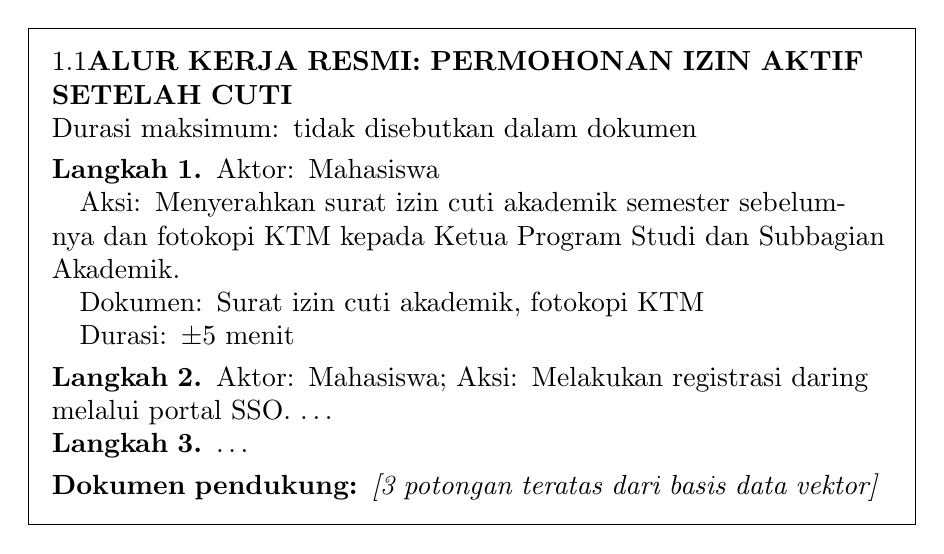
\begin{tikzpicture}
\node[draw, inner sep=3mm, text width=0.88\linewidth, align=left, font=\normalsize, execute at begin node=\setstretch{1.1}] {%
\textbf{ALUR KERJA RESMI: PERMOHONAN IZIN AKTIF SETELAH CUTI}\\
Durasi maksimum: tidak disebutkan dalam dokumen\\[3pt]
\textbf{Langkah 1.} Aktor: Mahasiswa\\
\hspace*{1em}Aksi: Menyerahkan surat izin cuti akademik semester sebelumnya dan fotokopi KTM kepada Ketua Program Studi dan Subbagian Akademik.\\
\hspace*{1em}Dokumen: Surat izin cuti akademik, fotokopi KTM\\
\hspace*{1em}Durasi: $\pm$5 menit\\[3pt]
\textbf{Langkah 2.} Aktor: Mahasiswa; Aksi: Melakukan registrasi daring melalui portal SSO. \dots\\
\textbf{Langkah 3.} \dots\\[3pt]
\textbf{Dokumen pendukung:} \textit{[3 potongan teratas dari basis data vektor]}};
\end{tikzpicture}
\caption{Contoh Blok Alur Kerja pada \textit{Prompt}}
\label{fig:prompt}
\end{figure}

\subsection{Perancangan Antarmuka Pemrograman Aplikasi}
Komunikasi antara E-Office dan layanan RAG menggunakan REST API dengan format JSON. Rancangan \textit{endpoint} ditunjukkan pada Tabel~\ref{tab:api}.

\begin{table}[htbp]
\caption{Rancangan \textit{Endpoint} REST API}
\label{tab:api}
\centering\tabsetup
\begin{tabularx}{\linewidth}{|C{0.6cm}|C{1.4cm}|L{4.2cm}|Y|}
\hline\hdr
\hrow\textbf{No} & \textbf{Metode} & \textbf{Endpoint} & \textbf{Fungsi} \\\hline
1 & POST & \code{/api/chat} & Mengirim pertanyaan dan menerima jawaban beserta sumber (E-Office) \\\hline
2 & GET & \code{/api/chat/history} & Mengambil riwayat percakapan pengguna (E-Office) \\\hline
3 & GET & \code{/api/letters/status} & Mengambil status surat milik pengguna (E-Office, dipanggil layanan RAG) \\\hline
4 & POST & \code{/rag/answer} & Menjalankan alur LangGraph untuk satu pertanyaan (layanan RAG) \\\hline
5 & POST & \code{/rag/reindex} & Membangun ulang graf alur kerja dan indeks vektor (layanan RAG, khusus admin) \\\hline
6 & GET & \code{/rag/health} & Memeriksa ketersediaan layanan RAG dan Ollama \\\hline
\end{tabularx}
\end{table}

\subsection{Perancangan Basis Data}
Basis data PostgreSQL E-Office ditambah dua tabel untuk menyimpan percakapan. Rancangan tabel ditunjukkan pada Tabel~\ref{tab:db}.

\begin{table}[htbp]
\caption{Rancangan Tabel Percakapan}
\label{tab:db}
\centering\tabsetup
\begin{tabularx}{\linewidth}{|C{0.6cm}|L{2.8cm}|L{3.0cm}|Y|}
\hline\hdr
\hrow\textbf{No} & \textbf{Tabel} & \textbf{Kolom} & \textbf{Keterangan} \\\hline
1 & \code{chat\_sessions} & \code{id}, \code{user\_id}, \code{created\_at} & Sesi percakapan milik pengguna \\\hline
2 & \code{chat\_messages} & \code{id}, \code{session\_id}, \code{role}, \code{content}, \code{sop\_id}, \code{route}, \code{latency\_ms}, \code{prompt\_tokens}, \code{created\_at} & Pesan pengguna dan asisten beserta SOP terpilih dan data kinerja \\\hline
\end{tabularx}
\end{table}

% ---------------------------------------------------------------------
\section{Implementasi}
\label{sec:implementasi}
Mesin \wgr{} diimplementasikan dalam Python dengan LangChain, LangGraph, NetworkX, dan Chroma, kemudian disajikan sebagai layanan REST. Implementasi melanjutkan kode penelitian pendahuluan dengan memindahkan setiap tahap ke simpul LangGraph. Rancangan fungsi pemilih SOP berdasarkan Persamaan~\ref{eq:skor} ditunjukkan pada Source Code~\ref{src:selector}.

\begin{sourcecode}{Rancangan fungsi pemilih SOP berbasis aturan}{src:selector}
def score(q: str, sop: dict) -> int:
    q = q.lower()
    s = 15 if sop["title"].lower() in q else 0
    for alias in sop["aliases"]:
        if alias in q:
            s += 8
        else:
            s += 2 * sum(w in q for w in alias.split() if len(w) > 2)
    if any(cue in q for cue in PROCEDURAL_CUES):
        words = {w for w in q.split() if len(w) > 4}
        s += sum(bool(words & set(st["action"].lower().split()))
                 for st in sop["steps"])
    return s

def select_sop(state: dict) -> dict:
    best = max(SOPS, key=lambda p: score(state["question"], p))
    s = score(state["question"], best)
    return {"sop_id": best["id"] if s >= 3 else None, "score": s}
\end{sourcecode}

Lingkungan implementasi ditunjukkan pada Tabel~\ref{tab:lingkungan}.

\begin{table}[htbp]
\caption{Lingkungan Implementasi}
\label{tab:lingkungan}
\centering\tabsetup
\begin{tabularx}{\linewidth}{|C{0.6cm}|L{4.0cm}|Y|}
\hline\hdr
\hrow\textbf{No} & \textbf{Komponen} & \textbf{Spesifikasi} \\\hline
1 & Perangkat keras & {[}diisi: prosesor, RAM, GPU server lokal{]} \\\hline
2 & Bahasa pemrograman & Python (mesin RAG), TypeScript (E-Office) \\\hline
3 & Mesin RAG & LangChain, LangGraph, NetworkX, Chroma, FastAPI \\\hline
4 & Model & \texttt{gemma4:e2b} melalui Ollama; \textit{embedding} \texttt{all-indo-e5-small-v4} \\\hline
5 & E-Office & Next.js, Bun, Elysia, PostgreSQL \\\hline
\end{tabularx}
\end{table}

% ---------------------------------------------------------------------
\section{Pengujian dan Evaluasi}
\label{sec:pengujian}
Subbab ini membahas sistem pembanding, prosedur evaluasi kualitas jawaban, pengujian \textit{black-box}, dan pengukuran efisiensi.

\subsection{Sistem Pembanding}
Sistem yang dibandingkan dalam evaluasi kualitas jawaban ditunjukkan pada Tabel~\ref{tab:sistem}. Seluruh sistem menggunakan model \textit{embedding}, parameter \textit{chunking}, basis data vektor, generator, dan templat \textit{prompt} yang sama agar perbedaan hasil hanya berasal dari cara konteks disusun.

\begin{table}[htbp]
\caption{Sistem Pembanding}
\label{tab:sistem}
\centering\tabsetup
\begin{tabularx}{\linewidth}{|C{0.6cm}|L{3.8cm}|Y|}
\hline\hdr
\hrow\textbf{No} & \textbf{Sistem} & \textbf{Konteks yang Diberikan kepada LLM} \\\hline
1 & LLM saja & Tanpa konteks; mengukur pengetahuan bawaan model \\\hline
2 & Naive RAG & Tiga potongan teratas hasil temu kembali padat \\\hline
3 & GraphRAG entitas & Tripel entitas satu lompatan ditambah tiga potongan teratas \\\hline
4 & \wgr{} & Blok alur kerja SOP terpilih ditambah tiga potongan pendukung \\\hline
5 & \textit{Selection-Matched Text} & Teks asli SOP terpilih ditambah tiga potongan pendukung (ablasi) \\\hline
6 & Konteks penuh & Seluruh 7 SOP \\\hline
7 & LightRAG & Graf entitas-relasi yang dibangun otomatis dengan LLM \parencite{guo2024lightrag} \\\hline
\end{tabularx}
\end{table}

Sistem nomor 1 sampai 6 mengikuti rancangan penelitian pendahuluan \parencite{wiratama2026procedure}, sedangkan LightRAG ditambahkan dalam skripsi ini untuk menguji apakah keunggulan \wgr{} tetap berlaku terhadap GraphRAG otomatis, bukan hanya terhadap graf entitas yang disusun manual.

\subsection{Prosedur Evaluasi Kualitas Jawaban}
Evaluasi kualitas jawaban dilakukan dengan langkah-langkah sebagai berikut:
\begin{enumerate}
\item Menjalankan setiap sistem pada 40 pertanyaan benchmark dengan temperatur generator 0.
\item Menghitung KFR dan ROUGE pada 35 pertanyaan yang dapat dijawab, cakupan langkah, TIR, dan AMR pada 11 pertanyaan prosedural, serta akurasi penolakan pada 5 pertanyaan di luar cakupan.
\item Memeriksa secara manual sampel baris penyelarasan langkah untuk mengukur kesesuaian penilai otomatis dengan penilaian manusia.
\item Menghitung \textit{faithfulness} dan \textit{answer relevancy} RAGAs sebagai bukti pendukung.
\item Menguji perbedaan antarsistem dengan uji Wilcoxon berpasangan dan koreksi Holm-Bonferroni.
\item Mengulangi evaluasi dengan satu LLM lokal pembanding untuk menguji kestabilan hasil terhadap pilihan generator.
\end{enumerate}

\subsection{Pengujian Black-Box}
Pengujian \textit{black-box} dilakukan untuk setiap kebutuhan fungsional pada Tabel~\ref{tab:fungsional}. Contoh rancangan skenario uji ditunjukkan pada Tabel~\ref{tab:blackbox}; daftar lengkapnya disajikan pada Lampiran 2.

\begin{table}[htbp]
\caption{Contoh Rancangan Skenario Pengujian \textit{Black-Box}}
\label{tab:blackbox}
\centering\tabsetup
\begin{tabularx}{\linewidth}{|C{0.6cm}|C{1.2cm}|L{4.0cm}|Y|}
\hline\hdr
\hrow\textbf{No} & \textbf{Kode} & \textbf{Skenario} & \textbf{Hasil yang Diharapkan} \\\hline
1 & F-02 & Mengirim ``bagaimana cara cuti kuliah?'' & SOP Izin Cuti Akademik terpilih \\\hline
2 & F-03 & Menanyakan prosedur legalisir ijazah & Enam langkah tampil berurutan dengan aktor yang benar \\\hline
3 & F-04 & Menanyakan aturan wisuda yang tidak ada dalam SOP & Sistem menolak dengan pesan bahwa informasi tidak tersedia \\\hline
4 & F-05 & Menanyakan ``surat saya sudah sampai mana?'' & Status surat terakhir pengguna, tahap berikutnya, dan aktornya tampil \\\hline
5 & F-07 & Membuka kembali halaman percakapan & Riwayat percakapan sebelumnya tampil \\\hline
\end{tabularx}
\end{table}

\subsection{Pengukuran Efisiensi}
Efisiensi diukur dari jumlah token \textit{prompt}, jumlah pemanggilan LLM, dan waktu respons untuk setiap pertanyaan. Waktu respons diukur dari saat \textit{backend} E-Office menerima pertanyaan sampai jawaban dikirim kembali, sehingga mencakup waktu temu kembali, pemanggilan LLM, dan komunikasi antarlayanan.

% ---------------------------------------------------------------------
\section{Jadwal Penelitian}
\label{sec:jadwal}
Jadwal pelaksanaan penelitian ditunjukkan pada Tabel~\ref{tab:jadwal}. % TODO: sesuaikan dengan tanggal seminar proposal

\begin{table}[htbp]
\caption{Jadwal Penelitian}
\label{tab:jadwal}
\centering\tabsetup
\newcommand{\x}{\cellcolor{g55}}
\begin{tabular}{|c|L{5.0cm}|C{1.05cm}|C{1.05cm}|C{1.05cm}|C{1.05cm}|C{1.05cm}|C{1.05cm}|}
\hline\hdr
\textbf{No} & \textbf{Kegiatan} & \textbf{Okt} & \textbf{Nov} & \textbf{Des} & \textbf{Jan} & \textbf{Feb} & \textbf{Mar} \\\hline
1 & Studi literatur dan pengumpulan data & \x & \x & & & & \\\hline
2 & Analisis kebutuhan & \x & \x & & & & \\\hline
3 & Perancangan sistem & & \x & \x & & & \\\hline
4 & Implementasi mesin RAG dan integrasi E-Office & & & \x & \x & & \\\hline
5 & Pengujian dan evaluasi & & & & \x & \x & \\\hline
6 & Penyusunan laporan & \x & \x & \x & \x & \x & \x \\\hline
\end{tabular}
\end{table}

% =====================================================================
\chapter{Hasil dan Pembahasan}
\label{bab:4}
% =====================================================================
% TODO: bab ini diisi setelah implementasi dan evaluasi. Kerangka di bawah
% mengikuti Bab III agar setiap rancangan memiliki hasil yang sesuai.
Bab ini membahas hasil implementasi asisten virtual, hasil pengujian \textit{black-box}, hasil evaluasi kualitas jawaban dan efisiensi, serta pembahasan terhadap hasil tersebut.

\section{Hasil Implementasi Graf Alur Kerja}
[Akan diisi: statistik graf, hasil verifikasi kutipan dan jumlah langkah.]

\section{Hasil Implementasi Asisten Virtual pada E-Office}
[Akan diisi: tampilan widget percakapan, contoh jawaban prosedural dan status surat.]

\section{Hasil Pengujian Black-Box}
[Akan diisi: tabel hasil pengujian setiap kebutuhan fungsional.]

\section{Hasil Evaluasi Kualitas Jawaban}
[Akan diisi: KFR, cakupan langkah, TIR, AMR, akurasi penolakan, RAGAs, dan uji statistik untuk setiap sistem pembanding.]

\section{Hasil Pengukuran Efisiensi}
[Akan diisi: token \textit{prompt} dan waktu respons.]

\section{Pembahasan}
[Akan diisi: jawaban atas rumusan masalah, perbandingan dengan penelitian terkait, dan keterbatasan.]

% =====================================================================
\chapter{Penutup}
\label{bab:5}
% =====================================================================
% TODO: diisi setelah Bab IV selesai.
Bab ini berisi kesimpulan yang diperoleh dari penelitian dan saran untuk pengembangan selanjutnya.

\section{Kesimpulan}
[Akan diisi.]

\section{Saran}
[Akan diisi.]


% =================== BAGIAN AKHIR ====================================
\printbibliography[heading=bibintoc,title={DAFTAR PUSTAKA}]
% =====================================================================
%  LAMPIRAN
% =====================================================================
\lampiran{Daftar Pertanyaan Benchmark}
[Akan diisi: 40 pertanyaan benchmark beserta kategori dan jawaban acuan.]

\lampiran{Tabel Pengujian Black-Box}
[Akan diisi: daftar lengkap skenario dan hasil pengujian.]


\end{document}
